% Do not forget to include Introduction
%---------------------------------------------------------------
% \chapter{Introduction}
% uncomment the following line to create an unnumbered chapter
\chapter*{Introduction}\addcontentsline{toc}{chapter}{Introduction}\markboth{Introduction}{Introduction}
%---------------------------------------------------------------
\setcounter{page}{1}

% The following environment can be used as a mini-introduction for a chapter. Use that anyway it pleases you (or comment it out). It can contain, for instance, a summary of the chapter. Or, there can be a quotation.
\begin{chapterabstract}
	Product configurators and their value.
\end{chapterabstract}

Over the past few decades, the rise of e-commerce has caused a shift in consumer expectations, resulting in an increased demand for customized products. This gives rise to the need to shift focus towards mass customization, where products are customized according to individual preferences. To thrive in this sector, companies must modify their product offerings to be able to meet the unique needs of users. This necessitates the existence of a system (a toolkit), that enables customers to express their preferences and convert them into product configurations. \cite{Fulkerson2000}

The introduction of customization has been shown to significantly improve the customer's perception of the product's value. The involvement of consumers in the customization process leads to a stronger bond with the product, resulting in a perception of higher value compared to standard off-the-shelf products. This aspect of mass customization makes it an appealing and compelling strategy for businesses to implement. \cite{Schreier2006} However, when implementing such a system, it is crucial to ensure that the customization process is pleasurable for the customer. Research has shown that the enjoyment experienced during the customization also affects the perceived value of the final product, highlighting the importance of good implementation. \cite{Franke2010}

The task of transforming user preferences into concrete designs is a difficult endeavor that can be further hindered by a lack of effective communication between the customer's explanation of their desires and the business's comprehension. The use of online product configurators seemingly provides a solution for this issue by offering a user-friendly and visually appealing platform, which allows customers to customize products to their specifications, improves customer experience by increasing engagement and interactivity, and helps to bridge the gap between customer expectations and the end product. These tools have become an integral part of successful personalization strategies. \cite{Franke2003}

The introduction of modern technologies such as WebGL or Augmented Reality (AR) has expanded the potential of online configurators. These advances enable these toolkits to become more powerful and visually illustrative tools that provide a higher level of interactivity and realism than what was previously accessible. \cite{Cozzi2015}

%---------------------------------------------------------------
\section{Objective of this thesis}
%---------------------------------------------------------------

The primary objective of this thesis is to design and implement an application (toolkit) for the online configuration of modular products. The toolkit aims to be product-agnostic, adaptable, and customizable, usable by various businesses, enabling their customers to customize their modular products interactively. The focus is on ensuring that the toolkit is not only flexible in accommodating various specific needs, but also straightforward for businesses to maintain after deploying, emphasizing lightweight infrastructure requirements. 
To accomplish this main objective, this requires an analysis of the characteristics found in current product configurators, as well as an examination of comparable solutions currently available to businesses.

%---------------------------------------------------------------
\section{Structure of this thesis}
%---------------------------------------------------------------

This thesis is divided into six chapters.

\begin{description}
\item[Chapter 1] The initial chapter entails an examination of existing solutions and an investigation into the functionalities that should be incorporated into this particular application.

\item[Chapter 2] The second chapter discusses the design of the application, the technologies chosen, the architecture, and the data structures.

\item[Chapter 3] The third chapter is devoted to implementation.

\item[Chapter 4] Chapter four focuses on the deployment of the implemented application in a particular business as an example. In addition, it discusses the resulting changes in the business processes of the selected business.

\item[Chapter 5] In the fifth chapter, the tests used in the development of the application are described.

\item[Chapter 6] Finally, the last chapter summarizes the results achieved and suggests possible directions for future development.
\end{description}


%---------------------------------------------------------------
\chapter{Analysis}
%---------------------------------------------------------------

\begin{chapterabstract}
	Lorem ipsum dolor sit amet. 
\end{chapterabstract}

Product configurators can be implemented in various ways, and the design of the tool itself determines the types of products that can be designed using the tool later on. The number of different unique configurations of a product that the tool can create is called the solution space. The size of the solution space is determined by two factors: the number of customizable attributes and the achievable values of each attribute. \cite{Huiwen2018} A relevant study examines the solution spaces of these toolkits and proposes an evaluation model that enables the categorization and assessment of various implementation approaches. Based on the target outcome and the guidance provided by the tool, the following mechanisms are specified: \cite{Hermans2012}

\begin{definition}[Veneer]
Customization by adding a visual decorative layer. (e.g. printing, engraving, etching)
\end{definition}
\begin{definition}[Modularity]
Customization by combining modules or components.
\end{definition}
\begin{definition}[Parametric]
Customization by changing the parameter values of parts.
\end{definition}
\begin{definition}[Generative]
Customization using code and scripting to synthesize the final form of the product.
\end{definition}

The main focus of this thesis is on toolkits that primarily employ modularity mechanisms, however, there are often some common characteristics among configuration tools with different mechanisms.

\section{Existing solutions}
\subsection{Applications of product configurators}

Currently, many companies are integrating product configurators into their sales strategies across multiple industries such as automotive, fashion, furniture, housing, and others. These configurators serve as either the main or supplementary sales tools for these businesses.

The Configurator Database Project by cyLEDGE MEDIA aims to catalog these web-based configuration tools. In the 2017/2018 report, they tracked 1250 deployments of these tools; however, the true count will be significantly higher since the database only includes the most frequently visited applications. \cite{cyLEDGE2018}

An analysis of the 100 most viewed configurators from May 2020 to May 2021 in the Configurator Database Project was performed in a study that examined the shared characteristics of these configurations. The results of some of the relevant characteristics and design choices that the study has analyzed are presented in this section: \cite{Blazek2023}
\begin{itemize}
    \item \textbf{Responsive design}: 75.3\% of examined tools had responsive design (the design adapted to the viewport of the device) 
    \item \textbf{Navigation}: 17.5\% of configurators had linear predefined navigation (meaning the configuration had to follow a specified sequence), whereas the majority of tools (82.5\%) had open navigation (user has the flexibility to configure the product in any order)
    \item \textbf{Visualization} 79.4\% of tools utilized photorealistic visualization (as opposed to illustrations or no visualization), however, the study acknowledges that there were significant variations based on the industries in which the configurator is utilized
    \item \textbf{Data transfer} The mean network data size transferred for 3D configurator was 35.6~MB
    \item \textbf{Configuration options} 60.8\% of configurators offered more than ten customizable attributes
    \item \textbf{Purchase capability} Given that car brands typically do not directly sell their cars online, it is logical to exclude them from the analysis of this particular characteristic. With the exclusion of vehicle configurators, 70.5\% of the configurators could complete an online purchase of the configured product
    \item \textbf{Price calculation} 56.7\% of the configurators were able to instantly reflect the changes made to the configuration in the displayed price
\end{itemize}

Another article also used the same database of configurators to analyze common design elements. They identified several key designs that were prevalent in the majority of configurators analyzed. The following key insights of common, recommended designs from the article are relevant to this thesis: \cite{Leitner2014}
\begin{itemize}
    \item At the end of the configuration process, a summary of selected options is presented
    \item To present the products that can be configured, images that are large enough to see details are used
    \item If the configurator has linear predefined navigation, the navigation information is presented on a horizontal plane
    \item Navigation bar is visible
    \item Price and order button is clearly visible and available for completion purposes
    \item Prices of the components are accessible in all phases of the configuration
    \item Logo is displayed prominently
\end{itemize}

As part of the analysis chapter of this thesis, it is essential to examine actual 3D~configurator applications. Due to the large number of existing applications, it is not within the scope of this work to perform an exhaustive analysis. Instead, this section will focus on a select group of three applications. These have been selected based on a combination of factors such as their popularity, functionality, and importance in the context of a modular product configuration. This selection is intended to provide insightful examples that highlight different approaches, rather than being representative of the entire domain.

\subsubsection{IKEA PAX Planner Tool}

IKEA is a widely recognized global home furnishings retailer specializing in affordable furniture. \cite{StatistaIkea}

IKEA offers the PAX wardrobe, which is an easily configurable fitted wardrobe, for which they not only sell predefined configurations but also allow customers to modularly choose the ideal size, doors, knobs, handles, interior organization, and lightning.

To accomplish this, they utilize the PAX planner web tool (3D configurator). \footnote{Available at: \url{https://www.ikea.com/addon-app/storageone/pax/web/latest/cz/en/}} 

\begin{figure}[h]
\centering
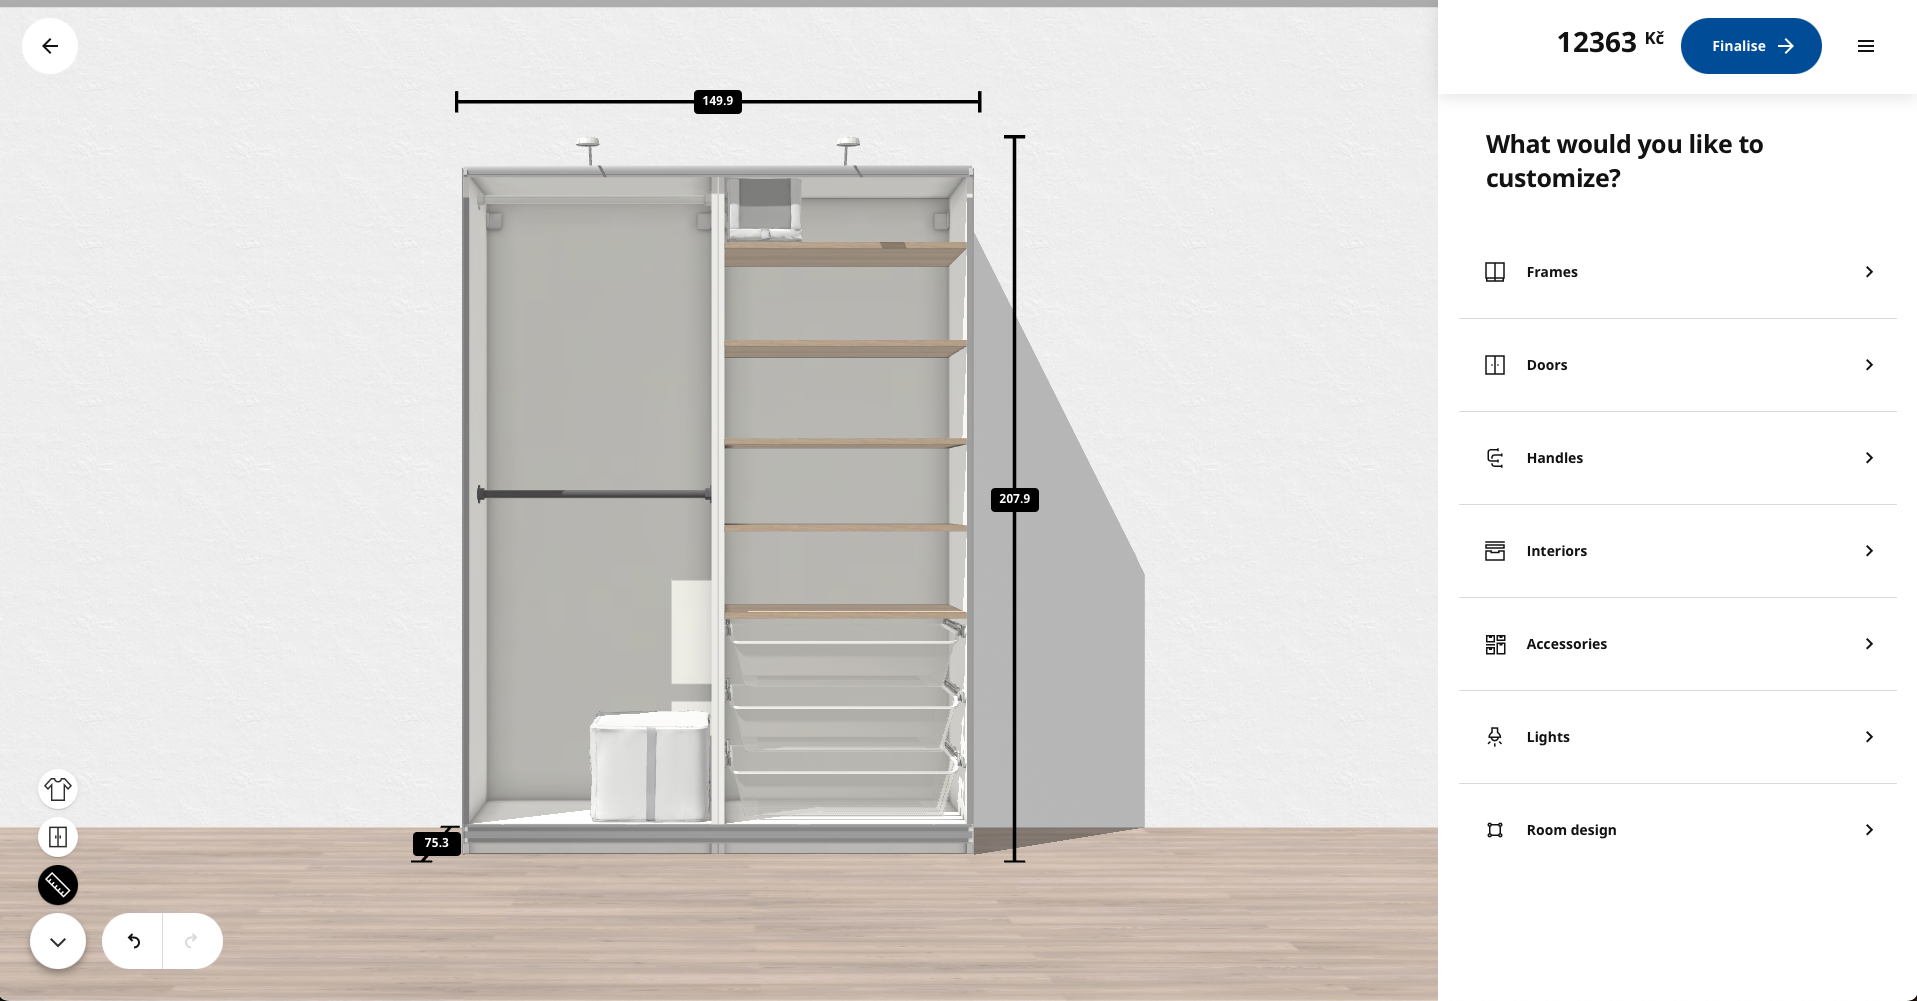
\includegraphics[width=14cm]{images/analysis_ikea-pax.png}
\caption{Screenshot of IKEA PAX Planner Tool with example configuration}
\end{figure}

The configurator has open navigation and consists mainly of two views. At the beginning of the process, the application prompts the user to select the starting point of the configuration. The main larger view provides a 3D view of the current configuration, allowing users to observe objects from different viewpoints by moving along an orbital trajectory around them. All options that can be chosen and added to the current configuration are found in the secondary window. Users can interact with elements in the 3D view. The layout of components can be adjusted in this way, and the selection of a component provides users with additional information and real-life images of the selected item.
The page is responsive, and the secondary window moves from the right side to a bottom sliding panel on mobile devices.
The tool performs live price calculations and contains a final summary confirmation screen with the option to order the configured product. The configurator is a single-page application (SPA is a web application implementation approach that loads only a single page and then sequentially updates the content of the page with scripting on the client side, rather than loading whole new pages from the server \cite{Fink2014}) and does not update the URL based on the selected product or phase of the configuration.

The configurator provides a range of creative features, such as the ability to change the visibility of some elements using a button (hiding the doors of a wardrobe to reveal the contents inside), the ability to display dimensions directly in the 3D view, undo and redo buttons, as well as the ability to save the configuration, which can be later loaded using generated code.

\subsubsection{Muuto Product Planner}

Muuto is a Scandinavian design company that produces furniture and home accessories. \cite{Muuto}

The company provides the Product Planner (3D web-based configurator), which allows customers to customize and combine the designs of various products, such as storage systems, sofas, tables, or wall hangers, tailored to their specific needs. \footnote{Available at: \url{https://planner.muuto.com/}}

\begin{figure}[h]
\centering
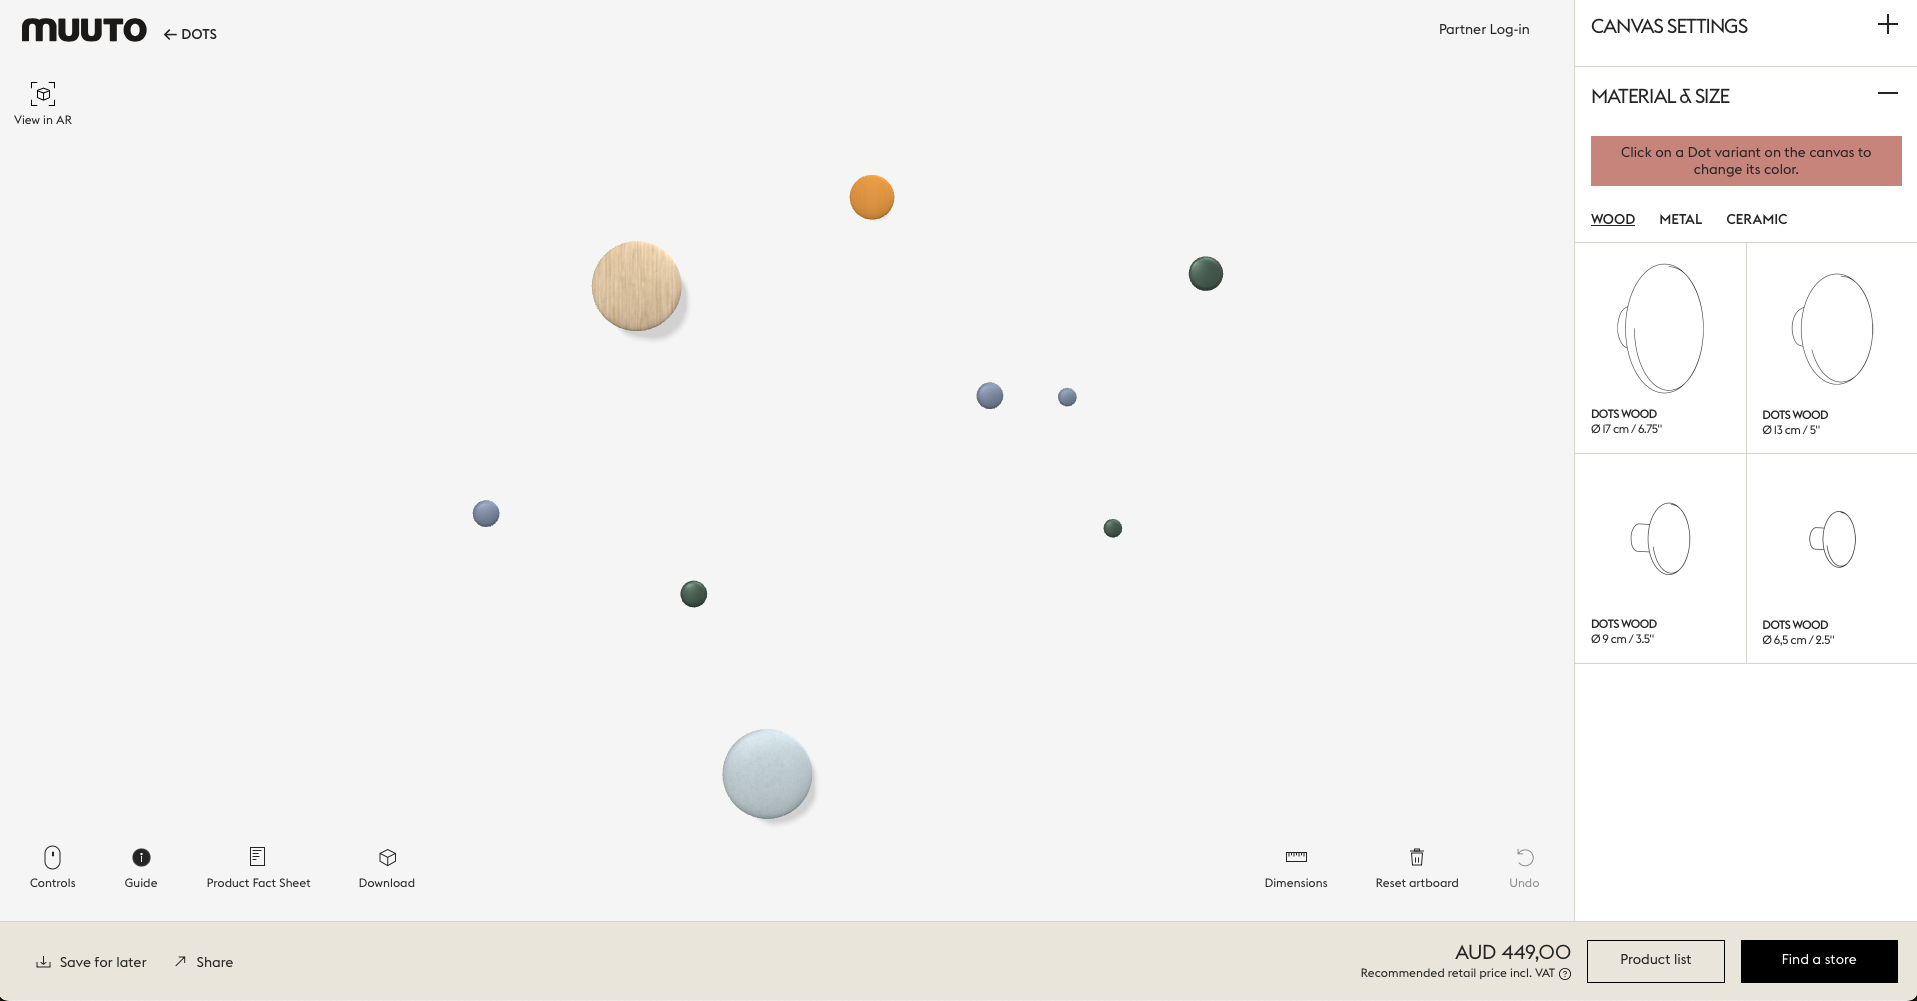
\includegraphics[width=14cm]{images/analysis_muuto-product-planner.png}
\caption{Screenshot of Muuto Product Planner tool with example configuration}
\end{figure}

The design of the configurator is similar to that in the previous case. The configurator also consists of two views and has open navigation. The primary views provide full 3D visualization, while the secondary views on the right side allow users to add components. On smaller devices, this secondary view transforms into a bottom slide panel, as the design is also responsive. The application follows a similar flow, starting with the selection of the starting point and then moving into the configurator. Live price calculation is also performed, and there is a summary page, but it is not possible to order the product, instead, the user is redirected to a physical store locator. In addition, there is also the possibility to display real dimensions and save the setup with distinct generated code, and the undo button allows one to revert previous actions.

In addition, the tool also has inventive functionalities. The designed configuration can be quickly shared with other users using email, or it can be downloaded, in several file formats containing the 3D model itself. The application allows to view the product in AR, directly in a web browser, albeit only on Apple devices using the Universal Scene Description (USDZ) format and AR~Quick Look. \cite{Jackson2018}
The application has multiple URL schemes that depend on the configuration phase, but they are not determined by the current product. 

Due to the wide variety of products that it supports, the configurator is not restricted to generating configurations that are feasible to produce and can create impossible configurations.

\subsubsection{LD Seating Nido configurator}

LD Seating is a company based in the Czech Republic that specializes in the production of chairs, armchairs, and sofas. \cite{LDSeating}

The company uses a 3D web-based configurator to market the Nido modular seating system, which consists of elements that are designed to be combined in various ways. \footnote{Available at: \url{https://nido.ldseating.com/en/configurator}}

\begin{figure}[ht]
\centering
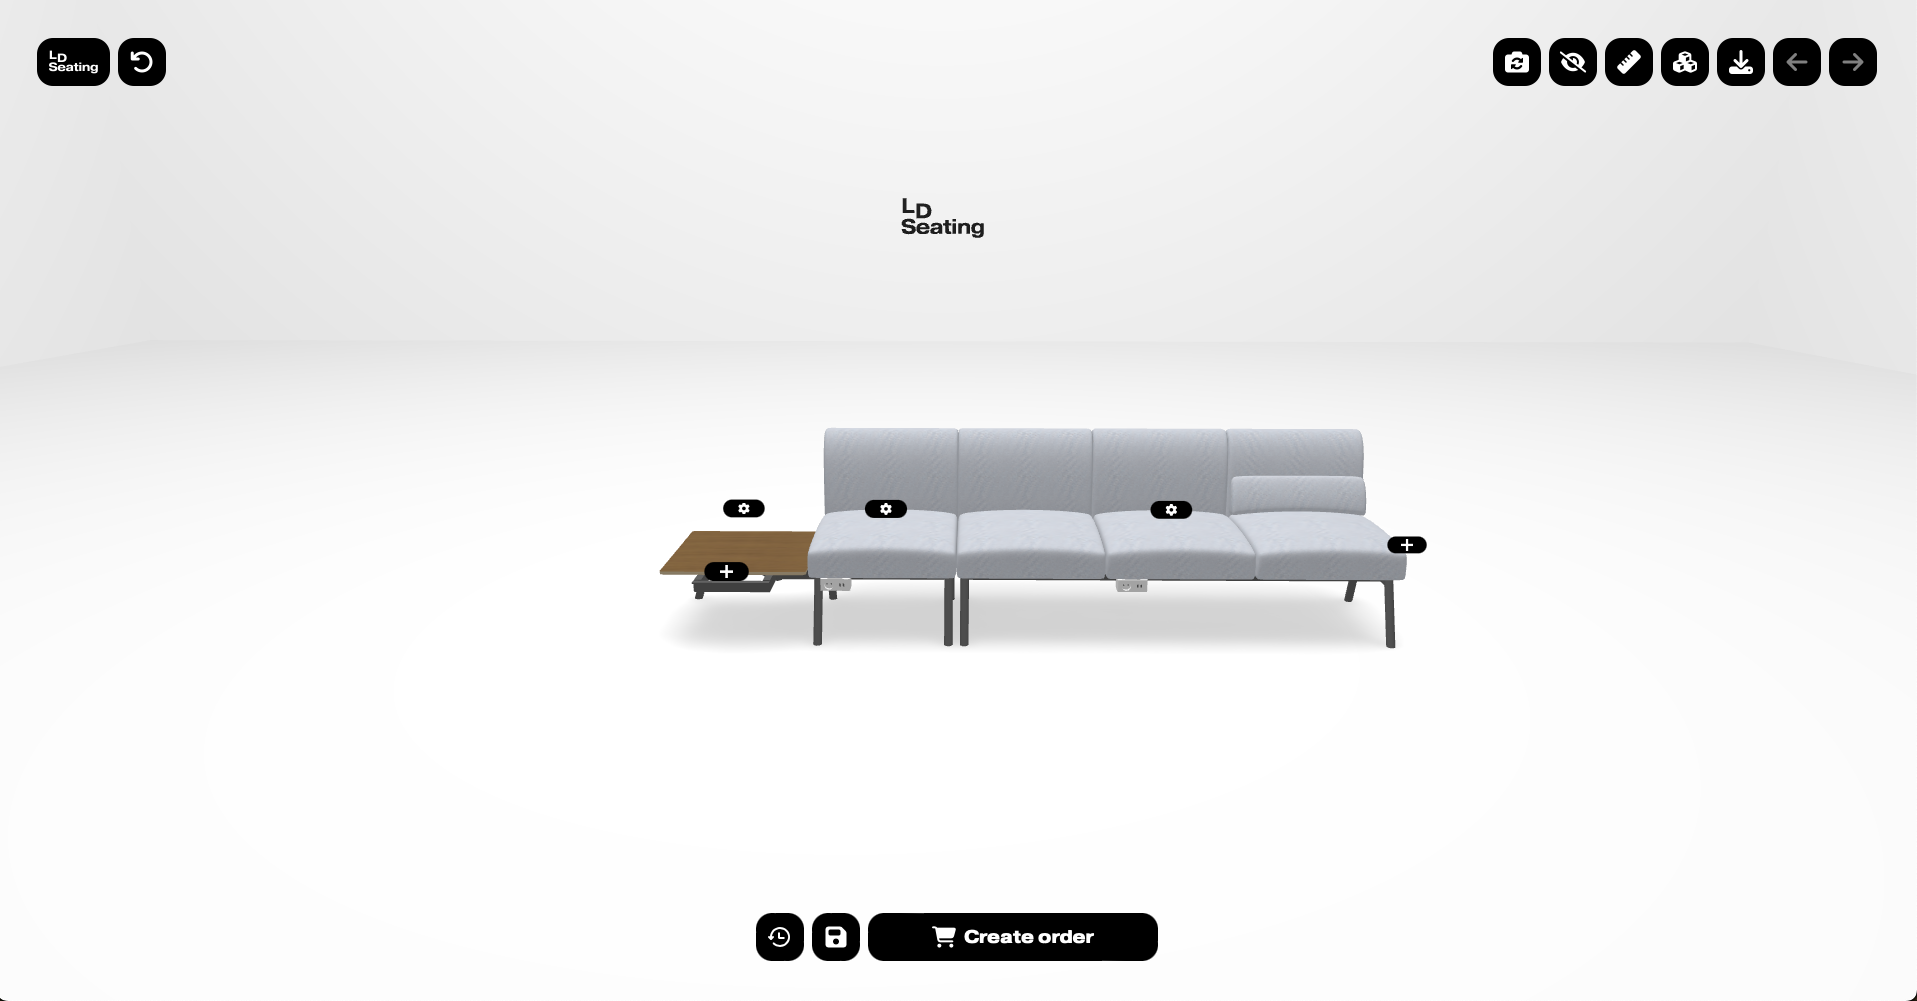
\includegraphics[width=14cm]{images/analysis_nido-configurator.png}
\caption{Screenshot of LD Seating Nido configurator with example configuration}
\end{figure}

The primary view of the configurator displays the 3D models of the components, and the flow of the application as well includes selecting a starting point, the product configuration itself, and a summary with confirmation. The controls for adding components and changing properties are integrated within the 3D scene itself. When user input is needed, a panel is opened on the right. The application is partially responsive, as the side panel does open in fullscreen on smaller viewports, however, there are some issues with image and text overflows on mobile devices. In this case, the configurator does not calculate the price and cannot directly place an order for the product but instead sends an inquiry for the configuration, and pressing the configuration confirmation results in displaying an inquiry form.

The tool has the ability to display dimensions, and the user can download the resulting configuration as a file that contains the 3D model. The configurator provides the option to save the configuration, and although it operates as an SPA, the saved configuration is then accessible at a specific URL containing the unique identification of the configuration. This feature also enables a version history mechanism.

\subsection{Available toolkits}

In this section of the analysis chapter, the focus shifts from specific 3D configurator applications to the fundamental toolkits that power the configurators. While many configurators are bespoke, tailored to the specific needs of individual companies and their products, sometimes even developed directly by the companies offering the products, there are providers offering more generic, adaptable solutions, aimed at companies that do not have the need, funds, or capabilities to develop a fully custom solution. These offerings are also highly relevant to this thesis, as the objective of this thesis is to create a product-agnostic toolkit, which means that there is a need to consider the way the configurator is set up by the business.

A variety of providers offer these toolkits for product configurators, with the aim of providing semi-custom or fully custom solutions, as well as generic options. To carry out a focused and relevant analysis, this section will examine two particular toolkits. The choice of toolkits analyzed has been complicated by the fact that most providers are quite cautious about the details of the technology, typically revealing in-depth information only after a serious business inquiry. The choice was also based on factors such as the implementation approach and compatibility with modular products.

\subsubsection{Threekit}

Threekit is a leading global company in visual commerce technologies that specializes in 3D product visualizations. The Threekit Platform, which enables clients to configure interactive product experiences according to their needs, functions as an administrative application and has the capability to generate product configurations. (see Figure \ref{fig:threekit-platform}) \cite{ThreeKitAboutUs} \cite{ThreeKitPlatform}

The platform is very complex with many distinct features. At its core, it uses a catalog for storing all product data (the products themselves, materials used, configurable parts, etc.). The items in the catalog can then be loaded into The Treekit Player, which will display the models in 3D, with the option for users to change attributes (models and materials) that are tied to the item. The behavior of the configurator can be set up using item rules and logic that support conditions, queries, and even custom scripts. The platform also offers a data tables feature that is similar to spreadsheets and is designed to handle extensive configuration data and logic. The application also has a built-in asset editor for refining 2D and 3D assets and configuration options. (see Figure \ref{fig:threekit-editor}) Models of the products can be uploaded in many 3D formats. The platform provides API integration with multiple business systems. \cite{ThreeKitPlatformDocumentation}

The offered solution is still partially tailored to the client, which is the reason why the service does not have standardized pricing. Instead, the price is determined through a personalized quote. It is important to note that the analysis of Threekit presented here is based on the publicly available documentation of the platform. Direct access to the full suite of Threekit's tools is typically available only after formalizing a business agreement with the company.

\subsubsection{Roomle}

Roomle is an Austrian company focused on pioneering visual product configuration. They provide solutions for product visualization, room design, and product configurators. Roomle's solution, called Rubens, is the "first Open Full Logic 3D-Configurator". The tool utilizes both parametric and modular mechanisms. The software allows integration with third parties through the use of an API. In addition, it supports front-end technologies on web and mobile platforms and has a built-in AR experience. \cite{RoomleAbout}

A web application, Rubens Admin, is used for setting up the configurator. To add a product which will then be configured by customers, 3D models and materials are uploaded to the admin application. Components are defined using the RoomleScript language, which is loosely based on the JavaScript language. The design of the configurator itself can be tuned in the admin application as well. Multiple language variants can be defined for product names and descriptions. The configurator application (see Figure \ref{fig:roomle}) runs on the client side and can be simply embedded into a website. Additionally, it can utilize a JavaScript library that can subscribe to events or modify the configurator. A framework is also provided to utilize the configurator within an iOS application. The client-side application fetches the configurable products from Google Cloud. \cite{RoomleDocumentation}

In terms of pricing, Roomle's Rubens configurator with the listed capabilities is offered to businesses at a monthly fee of 1450 euros. \cite{RoomleFullLogic}

\section{Proposed solution}

\subsection{Requirements}

\subsubsection{Functional requirements}
\subsubsection{Non-functional requirements}